
\textcolor{red}{Start with N-player version}

Consider an economy with $N$ agents, evolving in the time interval $[0,T]$.
Each agent is described at time $t$ by his wealth $A_t$ and his skill level $H_t$,
with $(A_t, H_t) \in \Omega = \mathbb{R} \times \mathbb{R}^+$ for every $t \in [0,T]$.
Agents control their consumption $c_t \in \mathbb{R}^+$, and the proportion of time they dedicate to working $u_t \in [0,1]$. 
We assume that the proportion $1 - u_t$ of time not used to working is used to improve their skill level. 

Each agent face the following optimization problem:
\begin{equation}
\begin{cases}
        \sup\limits_{(u,c) \in \mathcal{U} \times \mathcal{C}}\mathbb{E} [ \int_0^T f_c(c_s) + f_u(u_s) ds + Q(A_T) ], \text{ s.t.}\\
        d H_t = H^\xi_t g(1 - u_t) dt + \sigma_h H_t d W^h_t,\\
        d A_t = \left[ (\bar r_t - \delta) A_t + \bar w_t H_t u_t - c_t  \right] dt + \sigma_a A_t d W^a_t.
\end{cases}
\end{equation}


\textcolor{red}{explain term by term. Add table  for parameters.}

Suppose agents are distributed over $\Omega$ at time $t$ with a measure $\mu_t \in \mathcal{P}(\Omega)$.
Moreover, suppose that the production function $F$ for the economy depends on aggregate capital $\bar a$ and the effective supply of ability $\bar h^e$, and is given by a Cobb-Douglas function \cite{Add Refernce for Cobb-Douglas} as 
$$F(\bar a,\bar h^e) = k ({\bar a})^\beta ({\bar h^e})^{1-\beta}.$$

Given an measure flow $(\mu_t)_{t \in [0,T]}$ and a feedback form for the control $u: u(a,h), $, we can calculate the aggregate quantities
\begin{equation*}
    \begin{cases}
        \bar a_t = \int_\Omega a\, d\mu_t(a,h),\\
        \bar h^e_t = \int_\Omega u(a,h)\, h d\mu_t (a,h).
    \end{cases}
\end{equation*}
The value $\bar a_t$ is the average wealth of the economy, whereas $\bar h^e_t$ is the effective supply of skilled labor in the economy - note that the the integral term is a weighted average of the skill $h$ level over the population distribution $\mu_t$, where the weights $u(a,h)$ are the proportion of time an agent with wealth $a$ and skill level $h$ devotes to work.

At economic equilibrium, the interest rate and wage per time per ability satisfy
$$\bar r_t = \partial_a F(\bar a_t, \bar h^e_t),\quad \bar w_t = \partial_h F(\bar a_t, \bar h^e_t).$$
\textcolor{red}{analyze monotonicity and convexity wrt. aggregate quantities}


Solutions for \eqref{education_model:mfg_analytic_system} describe Nash equilibria for the mean-field limit of the game.
The function $V: [0,T] \times \Omega \mapsto \mathbb{R}$ is the value function for the game at the Nash equilibrium,
whereas the probability measure flow $\mu: [0,T] \times \Omega \mapsto \mathbb{R}$ describe the time evolution of the  population density over the state space $\Omega$.
\begin{equation}\label{education_model:mfg_analytic_system}
    \begin{cases}
        \partial_t V + (\bar r  - \delta) a \partial_a V + \HH_u  + \HH_c + \frac{1}{2} \sigma_a^2 a^2 \partial_{aa} V + \frac{1}{2} \sigma^2_h h^2 \partial_{hh} V = 0,\\
        \partial_t \mu + \partial_a \left( \left[ (\bar r - \delta) a + \partial_p \HH_u + \partial_p \HH_c \right] \mu \right)  + \partial_h \left( \partial_q \HH_u\, \mu\right)  - \frac{1}{2} \sigma_a^2 \partial_{aa} (a^2\mu) - \frac{1}{2} \sigma^2_h \partial_{hh} (h^2\mu) = 0,\\
        \mu(0,a,h) = \mu_0,\quad V(T,a,h) = Q(a)
    \end{cases}
\end{equation}
where
\begin{equation}
    \begin{cases}
        \HH_u(h,p,q) = \sup\limits_{u} \left \{ h^\xi \, g(1 - u)\, q + h u \, \bar w (\mu)\, p + f_u(u)\right\},\\
        \HH_c(p) = \sup\limits_{c} \left \{  f_c(c) - c \, p \right \}
    \end{cases}
\end{equation}

\subsection{Numerical Illustration}
        A deterministic, simplified version of the model was simulated through Picard iterations.
        
        \textcolor{red}{describe in more details what you did.}
        
        We aim to use this simulation as a benchmark for further studies.        
        Let's set \textcolor{red}{Parameter table}
        $$g(1- u) = (1 - u),\,\xi = 0,\, \delta = 0.05, \, k = 0.5,\, f_c(c) = \log(c), f_u(u) = -\frac{\alpha}{2} u^2, Q(a) = a.$$        
        In this case, we have 
        \begin{equation}
            \begin{cases}    
            \HH_u(h,p,q) = \sup\limits_{u} \left\{ (1 - u)q + \bar w_t h u p - \frac{\alpha}{2} u^2 \right\},\\
            \HH_c (p) = \sup\limits_{c} \left\{ \log(c) - cp \right\}.
            \end{cases}
        \end{equation} 
        Two scenarios are simulated: $\alpha = 0.5$ and  $\alpha = 2$ representing a lower and a higher preference to education versus work, respectively.

        \textcolor{red}{Try to solve PDEs using DGM}
        \textcolor{red}{Change format of plots to suit document.}
        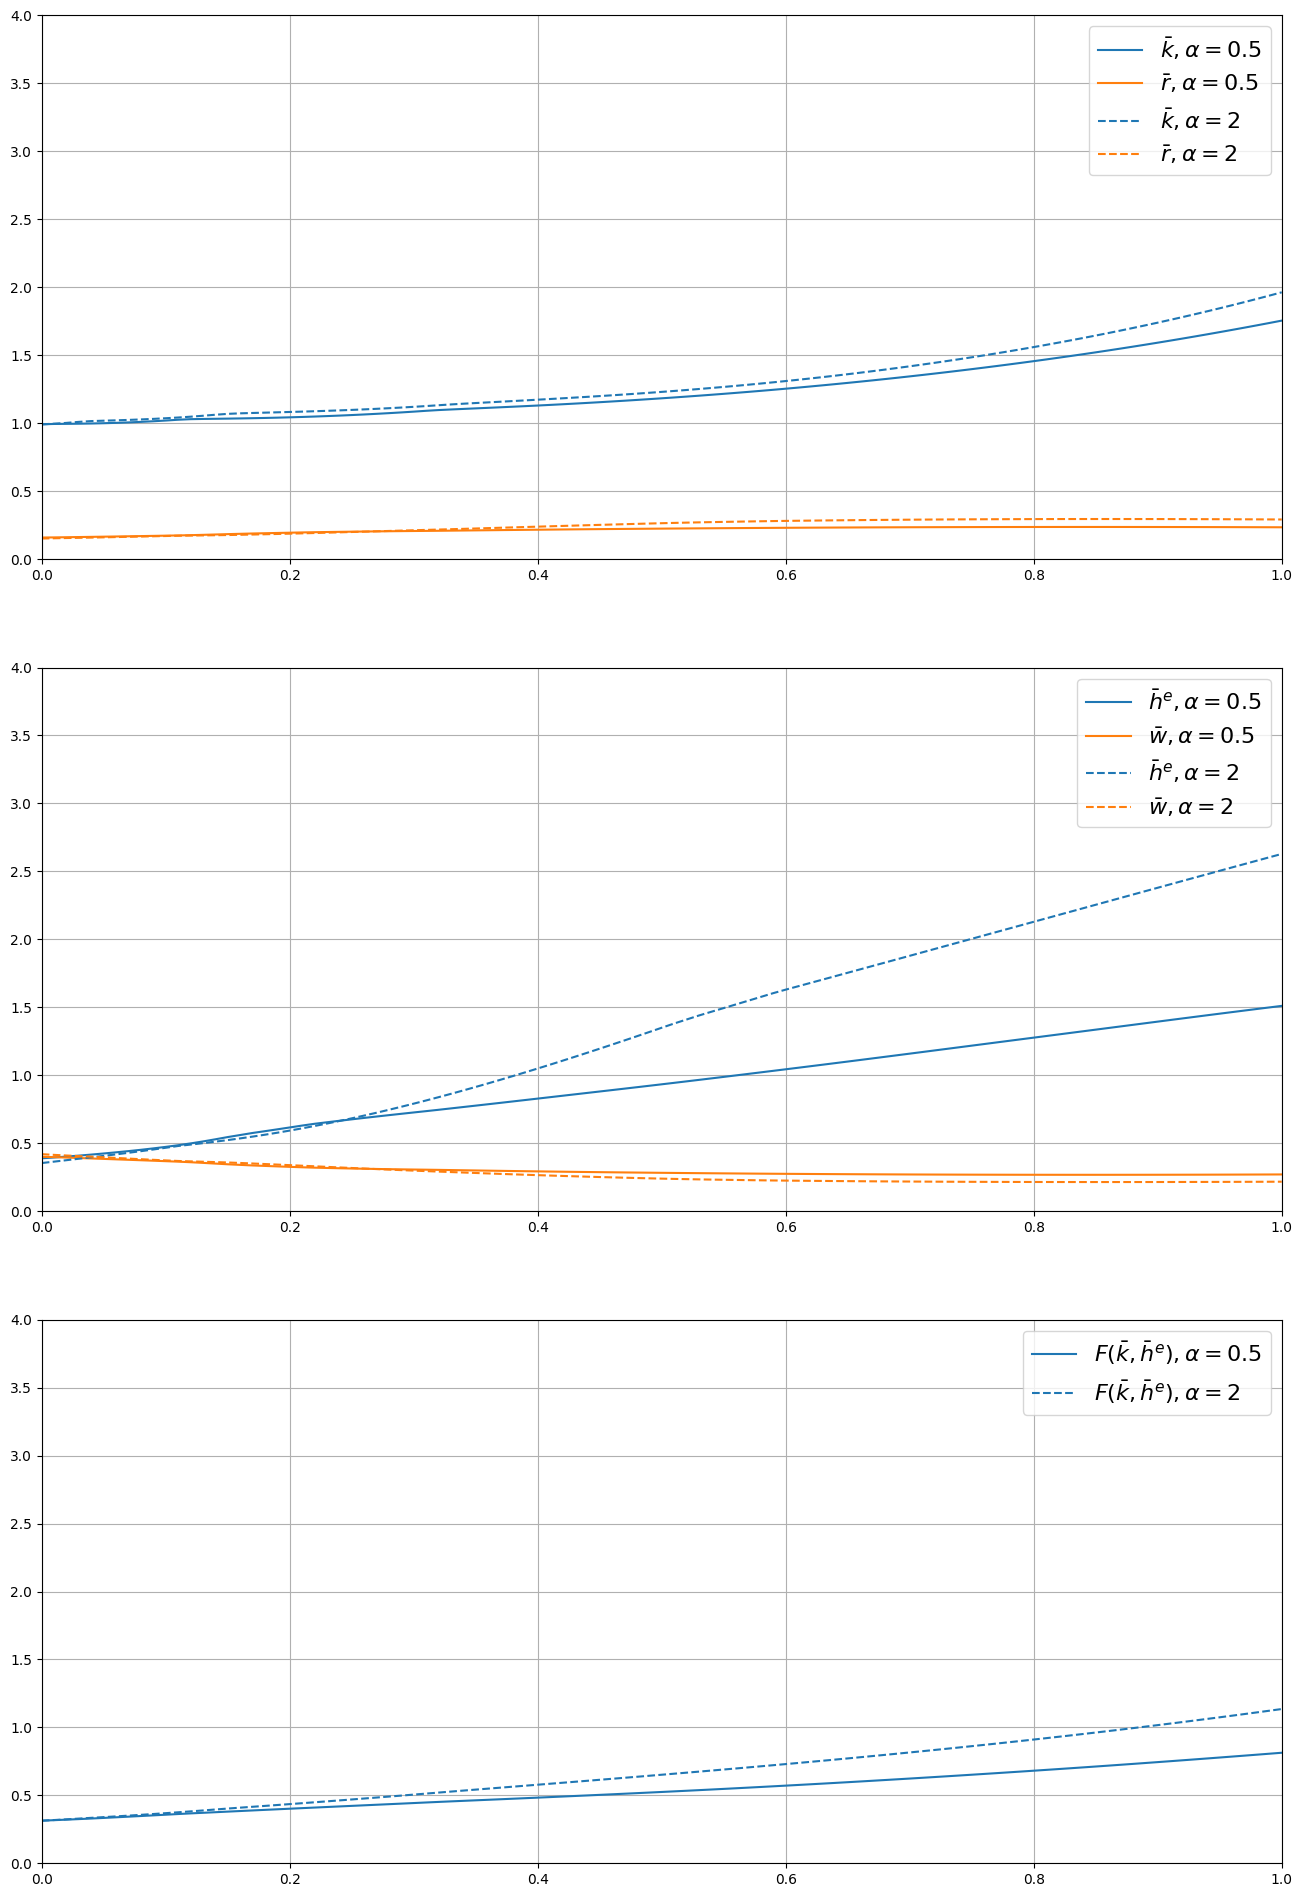
\includegraphics[width=\textwidth]{simulations_mfg.png}